

De methode valt uiteen in twee delen: Het bepalen van de t-90\% van een inverter en het bepalen van de t-90\% van drie inverters in cascade. 
\begin{enumerate}
\item Voor de eerste simulatie is het circuit in \ref{E1} gebruikt. De opdracht was om een enkele inverter te tekenen met een C\tss{load} van 25pF. Vervolgens diende deze gesimuleerd te worden bij een veranderende V6. Hierop moet dan een scope gezet worden om het ingangssignaal direct te zien. Bij "simulation parameters" dient dan een transient analyse aangevinkt te worden, om tegen de tijd te simuleren. De resultaten hiervan staan onder het kopje resultaten. 

\begin{figure} [h!]
\centering
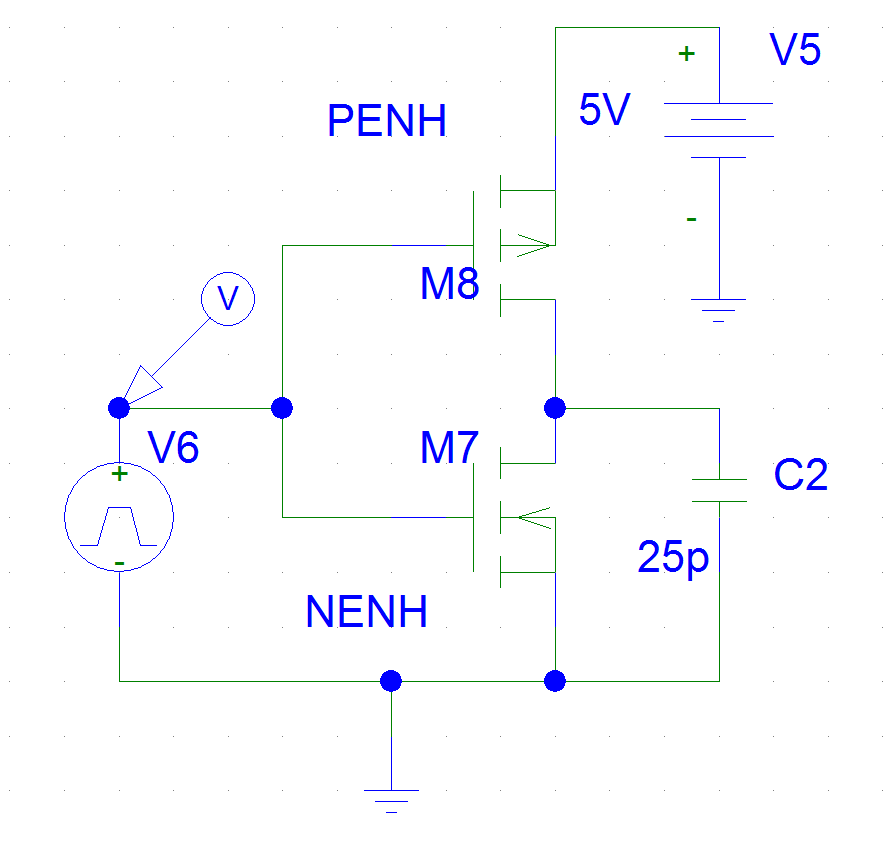
\includegraphics [scale = 0.4] {inputfiles/Inverter_circuit}
\caption{Het circuit van de enkele inverter in SPICE}
\label{E1}
\end{figure}
\newpage
\item Voor de tweede simulatie werd gevraagd om 3 inverters te simuleren. De eerste inverter is een normale inverter volgens de library die bij de opdracht gegeven is. De tweede inverter heeft een 5 keer zo grote breedte dan de eerste inverter en de derde inverter heeft een $5^2$ keer zo grote breedte als de eerste transistor. De bedoeling is dan om te onderzoeken of deze schakeling een bufferende werking heeft. De schakeling die hiervoor ontworpen is, staat in figuur \ref{E2}. De resultaten van de simulatie worden,  zoals eerder gezegd, hieronder besproken. 
\begin{figure} [h!]
\centering
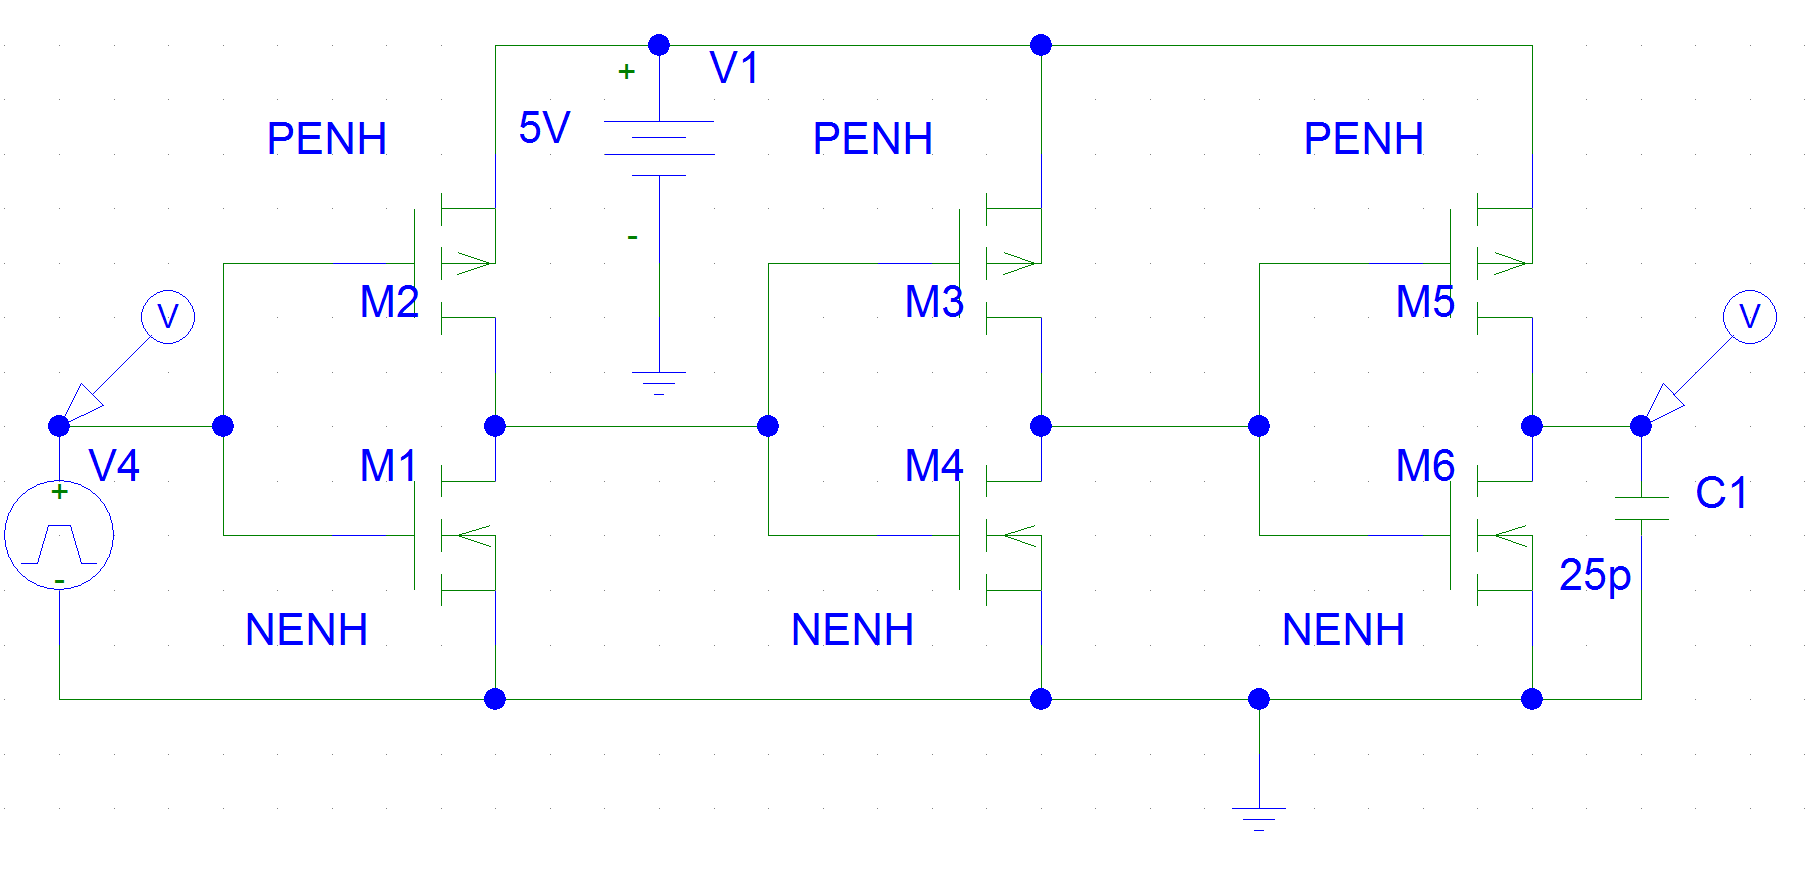
\includegraphics [width = \textwidth] {inputfiles/Cascade_circuit}
\caption{Het circuit van de driedubbele inverter in SPICE}
\label{E2}
\end{figure}
\end{enumerate}

